
\documentclass[a4]{beamer}
\usepackage{amssymb}
\usepackage{graphicx}
\usepackage{subfigure}
\usepackage{newlfont}
\usepackage{amsmath,amsthm,amsfonts}
%\usepackage{beamerthemesplit}
\usepackage{pgf,pgfarrows,pgfnodes,pgfautomata,pgfheaps,pgfshade}
\usepackage{mathptmx} % Font Family
\usepackage{helvet} % Font Family
\usepackage{color}
\mode<presentation> {
\usetheme{Default} % was Frankfurt
\useinnertheme{rounded}
\useoutertheme{infolines}
\usefonttheme{serif}
%\usecolortheme{wolverine}
% \usecolortheme{rose}
\usefonttheme{structurebold}
}
\setbeamercovered{dynamic}
\title[MA4704]{Technology Maths 4 \\ {\normalsize Lecture 11A}}
\author[Kevin O'Brien]{Kevin O'Brien \\ {\scriptsize kevin.obrien@ul.ie}}
\date{Spring 2013}
\institute[Maths \& Stats]{Dept. of Mathematics \& Statistics, \\ University \textit{of} Limerick}
\renewcommand{\arraystretch}{1.5}
%----------------------------------------------------------------------------------------------------------%
\begin{document}

\begin{frame}
\titlepage
\end{frame}



%---------------------------------------------------------------------%
\begin{frame}
\frametitle{Bivariate Data}
\begin{itemize}
\item Very often we are interested in the relationship between two
variables.
\item For example we might be interested in the relationship between
unemployment and inflation.
\item The investigation of a relationship between two variables
begins with an attempt to discover the approximate form of the
relationship by graphing the data using a scatter plot.
\end{itemize}	
\end{frame}
%---------------------------------------------------------------------%
\begin{frame}
\frametitle{Bivariate Data}
\begin{itemize}
\item  A scatter plot is a two-dimensional plot showing the (x,y) value for each
observation.

\item  Using these plots, we can quickly determine whether there is
any pronounced relationship and if so, whether the relationship may be
treated as approximately \textbf{linear}.\\
\begin{itemize}
\item Response variable Y (dependent variable).\\
\item Predictor variable X (independent variable).
\end{itemize}
\item A response variable is the variable whose variation we wish to explain.
\item The predictor variable is a variable used to explain the variation in the
response variable.
\end{itemize}	
\end{frame}
%---------------------------------------------------------------------%
\begin{frame}
\frametitle{Bivariate Data}
\begin{itemize}
\item The first step in determining the relationship between two
variables is to draw a \textbf{scatter plot}.
\item After establishing that a linear relationship exists between the
two variables X and Y, we need to measure the strength of this
relationship.
\item In order to do this, we need some measure of the association
or relationship between the two variables.
\item There are several ways of doing this - the most common
measure is the Pearson product moment correlation
coefficient usually known as the correlation coefficient.

\end{itemize}	
\end{frame}

\begin{frame}
\frametitle{Inspecting Scatter Plots (1) }
\begin{figure}
  % Requires \usepackage{graphicx}
  \includegraphics[scale=0.7]{11BPlot1.jpg}\\
\end{figure}
Relatively strong positive relationship (as height increases
weight on average increases), reasonably linear.

\end{frame}
\begin{frame}
\frametitle{Inspecting Scatter Plots (2) }
\begin{figure}
  % Requires \usepackage{graphicx}
  \includegraphics[scale=0.7]{11BPlot2.jpg}\\
\end{figure}

No relationship (at a stretch, a very weak negative relationship).
\end{frame}
\begin{frame}
\frametitle{Inspecting Scatter Plots (3) }
\begin{figure}
  % Requires \usepackage{graphicx}
  \includegraphics[scale=0.7]{11BPlot3.jpg}\\

\end{figure}

Negative, very strong, non-linear relationship
\end{frame}

\begin{frame}
\frametitle{Inspecting Scatter Plots (4) }
\begin{figure}
  % Requires \usepackage{graphicx}
  \includegraphics[scale=0.7]{11BPlot4.jpg}\\
\end{figure}
Non- Linear Relationship
\end{frame}

\begin{frame}
\frametitle{Outliers}
\begin{itemize}
\item A scatter plot may also be used to find outliers. These are
observations that do not fit the pattern of the remaining data.
\item Outliers may be due to mistakes in recording data.
\item To check the sensitivity of analysis to such outliers, analysis should
be carried out both with and without these outliers.
\end{itemize}
\end{frame}





%---------------------------------------------------------------------%
\begin{frame}
\frametitle{Correlation Coefficient}
\begin{itemize}
\item A correlation coefficient is a number between -1 and 1 which measures the degree to which two variables are \textbf{linearly} related. If the relationship in non-linear, then this measure is misleading.
\item The true correlation between two populations of values is denoted $\rho_{XY}$, and is almost always unknown. $\rho_{XY}$ is estimated by the estimate value $r_{XY}$, which is based on sample data.
\item If there is perfect linear relationship with positive slope between the two variables, we have a correlation coefficient of 1; if there is positive correlation, whenever one variable has a high (low) value, so does the other. 
\end{itemize}
\end{frame}

%---------------------------------------------------------------------%
\begin{frame}
\frametitle{Correlation Coefficient}
\begin{itemize}
\item If there is a perfect linear relationship with negative slope between the two variables, we have a correlation coefficient of -1; if there is negative correlation, whenever one variable has a high (low) value, the other has a low (high) value.
        
\item A correlation coefficient of 0 means that there is no linear relationship between the variables.
\item There are a number of different correlation coefficients that might be appropriate depending on the kinds of variables being studied.
\end{itemize}
\end{frame}

%---------------------------------------------------------------------%
\begin{frame}
\frametitle{Correlation Coefficient : Summations}

\begin{figure}
  % Requires \usepackage{graphicx}
  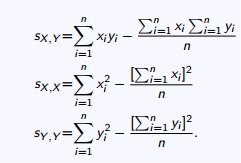
\includegraphics[scale=0.7]{11Bpearson.jpg}\\
  \caption{Summations}\label{11bpear}
\end{figure}
\end{frame}
%---------------------------------------------------------------------%
\begin{frame}
\frametitle{Correlation Coefficient : Formula}
The estimate of the Pearson correlation coefficient is given by
\[ r_{XY} = \frac{S_{XY}}{\sqrt{S_{XX}S_{YY}}} \]
\end{frame}
%---------------------------------------------------------------------%
\begin{frame}
\frametitle{Properties of the Correlation Coefficient}
\begin{enumerate}
\item $-1 \leq r \leq +1$
\item r = +1 or -1 represents a perfect positive linear correlation or a perfect negative linear
relationship between the variables.
\item r = 0 indicates little or no relationship i.e. as X increases there is no
definite tendency for the value of Y to increase or decrease in a straight line.
\item r close to +1 indicates a large positive correlation i.e. Y tends to increase
as X increases.
\item r close to -1 indicates a large negative correlation i.e. Y tends to decrease
as X increases.
\item The more r differs from 0, the stronger the linear relationship between the
two variables.
\item The sign of r indicates the direction of the relationship.
\end{enumerate}
\end{frame}


\begin{frame}
\frametitle{Correlation Coefficients (1) }
\begin{figure}
  % Requires \usepackage{graphicx}
  \includegraphics[scale=0.7]{11BPlot1.jpg}\\

\end{figure}
$r_{xy} = 0.87$ Strong Positive Linear Relationship

\end{frame}
\begin{frame}
\frametitle{Correlation Coefficients (2) }
\begin{figure}
  % Requires \usepackage{graphicx}
  \includegraphics[scale=0.7]{11BPlot2.jpg}\\

\end{figure}

$r_{xy} = -0.258$ (Almost) No Relationship
\end{frame}
\begin{frame}
\frametitle{Correlation Coefficients (3) }
\begin{figure}
  % Requires \usepackage{graphicx}
  \includegraphics[scale=0.7]{11BPlot3.jpg}\\

\end{figure}

$r_{xy} = -0.954$ Strong, though clearly non-linear
\end{frame}

\begin{frame}
\frametitle{Correlation Coefficients (4) }
\begin{figure}
  % Requires \usepackage{graphicx}
  \includegraphics[scale=0.7]{11BPlot4.jpg}\\

\end{figure}
$r_{xy} =  -0.051$ (although there is a very strong
relationship)
\end{frame}

%---------------------------------------------------------------------%
\begin{frame}
\frametitle{Correlation}
\begin{itemize}
\item This is a measure of Strength of Linear Relationship.
The correlation estimate is defined to be between -1 and 1.
\item It is not possible to have a correlation value outside this range of values
Additionally correlation estimates are not denominated in any units. (Contrast this to standard deviation, which is denominated in the same units as the mean ) .
\item A strong positive linear relationship describes a relationship between two variables whereby an increase in one variable will closely coincide with an increase in the other variable.
\item Conversely a strong negative linear relationship describes a relationship whereby an increase in one variable closely coincides with a decrease in the other.
\end{itemize}
\end{frame}
%-----------------------------------------------------%

%\frametitle{Outliers}
%Outliers can greatly influence the computed value of an estimate.
%Correlation is closely related to Simple linear regression models, in that both are concerned with the linear relationship between variables. However Linear Regression has a different emphasis.
%Simple Linear Regression describes one independent variable (IV) and the response of the dependent variable (DV).
%\end{frame}


\begin{frame}
\frametitle{Correlation and Causality }

\begin{itemize}
\item Note that a strong relationship between two variables does not
imply a cause-effect relationship.
For example, there is a strong negative correlation between the
sales of ice cream and the number of flu infections.
\item This does not mean that ice cream protects against flu.
\item This relationship results from a latent variable (a variable that has
not been observed).
\item Such a latent variable in this case is the weather. Low
temperatures and wet weather result in a high number of flu
infections and low ice cream sales. Hot, sunny weather leads to the
opposite.
\end{itemize}
\end{frame}

\begin{frame}
\frametitle{Pearson's Product Moment Correlation Coefficient}
\begin{itemize}
\item Pearson's product moment correlation coefficient, usually denoted by r, is just one example of a correlation coefficient.
\item However, these make the implicit assumption that the two variables are jointly normally distributed.
When this assumption is not justified, a non-parametric measure such as the Spearman Rank Correlation Coefficient might be more appropriate.
\end{itemize}
\end{frame}
\begin{frame}
The height of a boy was observed at 7 different ages.
Comment on the relationship between height and age over this
period of time and calculate the Pearson correlation coefficient for
this data.
\begin{figure}
  % Requires \usepackage{graphicx}
  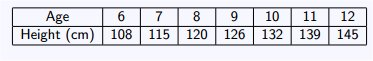
\includegraphics[scale=0.6]{11Bdata.jpg}\\

\end{figure}
X (the predictor variable) is defined to be age and Y is defined
to be height (the dependent variable).
\end{frame}
\end{document}
%---------------------------------------------------------------------%
%---------------------------------------------------------------------%
\begin{frame}
\frametitle{Properties of the Correlation Coefficient}
Example: We are given data for 6 graduates. Below is their
final QCA and their corresponding starting salary after
graduation.
\begin{tabular}{|c|c|c|c|c|c|c|}
  \hline
 Subject & 1 &2 &3 &4 &5 &6\\
 Final QCA &2.8& 3.4& 3.2& 3.8& 3.2& 3.4\\
 Starting Salary &20 000 &24 500& 23 000& 25 000 &20 000 &22 500\\
  \hline
\end{tabular}


Calculate the sample correlation coefficient.
\end{frame}

%---------------------------------------------------------------------%
\begin{frame}
\frametitle{Regression}
A statistical measure that attempts to determine the strength of the relationship between one dependent variable
(usually denoted by Y) and a series of other changing variables (known as independent variables).

Regression takes a group of random variables, thought to be predicting Y, and tries to find a mathematical relationship between them. This relationship is typically in the form of a straight line (linear regression) that best approximates all the individual data points.

\end{frame}


%---------------------------------------------------------------------%
\begin{frame}
\frametitle{Regression}

Two events can consistently correlate with each other but not have any causal relationship.
An example is the relationship between reading ability and shoe size across the whole population of the United States.
If someone performed such a survey, they would find that the larger shoe sizes correlate with better reading ability, but
this does not mean large feet cause good reading skills. Instead it's caused by the fact that young children have small
feet and have not yet (or only recently) been taught to read. In this case, the two variables are more accurately correlated with a third: age.
\end{frame}

\begin{frame}
\frametitle{Least Squares}
The method of least squares is a criterion for fitting a specified model to observed data.
For example, it is the most commonly used method of defining a straight line through a set of points on a scatterplot.
\end{frame}
%---------------------------------------------------------------------%
\begin{frame}
\frametitle{Regression Equation}
A regression equation allows us to express the relationship between two (or more) variables algebraically. It indicates the nature of the relationship between two (or more) variables. In particular, it indicates the extent to which you can predict some variables by knowing others, or the extent to which some are associated with others.



A linear regression equation is usually written
\[Y = a + bX + e\]
where
\begin{itemize}
\item Y is the dependent variable
\item a is the intercept
\item b is the slope or regression coefficient
\item X is the independent variable (or covariate)
\item e is the error term
\end{itemize{
The equation will specify the average magnitude of the expected change in Y given a change in X.

The regression equation is often represented on a scatterplot by a regression line.
\end{frame}

%---------------------------------------------------------------------%
\begin{frame}
\frametitle{Regression Line}

A regression line is a line drawn through the points on a scatterplot to summarise the relationship between the variables being studied. When it slopes down (from top left to bottom right), this indicates a negative or inverse relationship between the variables; when it slopes up (from bottom right to top left), a positive or direct relationship is indicated.

The regression line often represents the regression equation on a scatterplot.

\end{frame}

%---------------------------------------------------------------------%
\begin{frame}
\frametitle{Types of Regression}

\begin{itemize}
\item \textbf{Simple Linear Regression}
Simple linear regression aims to find a linear relationship between a response variable and a possible predictor variable by the method of least squares.



\item \textbf{Multiple Regression}
Multiple linear regression aims is to find a linear relationship between a response variable and several possible predictor variables.



\item \textbf{Nonlinear Regression}
Nonlinear regression aims to describe the relationship between a response variable and one or more explanatory variables in a non-linear fashion.
\end{itemize}
\end{frame}
%---------------------------------------------------------------------%
\begin{frame}
\frametitle{Residual}
Residual (or error) represents unexplained (or residual) variation after fitting a regression model.
It is the difference (or left over) between the observed value of the variable and the value suggested by the regression model.
\end{frame}

%---------------------------------------------------------------------%




\end{document} 